%%%%%%%%%%%%%%%%%%%%%%%%%%%%%%%%%%%%%%%%%%%%%%%%%%%%%%%%%%%%%%%%%%%%%%%
%%%%%%%%%%%%%%%%%%%%%%%%%%%%%%%%%%%%%%%%%%%%%%%%%%%%%%%%%%%%%%%%%%%%%%% 
%%%%%%%%%%%       								 Preamble				         	                                                        %%%%%%%%%% 
%%%%%%%%%%%%%%%%%%%%%%%%%%%%%%%%%%%%%%%%%%%%%%%%%%%%%%%%%%%%%%%%%%%%%%% 
%%%%%%%%%%%%%%%%%%%%%%%%%%%%%%%%%%%%%%%%%%%%%%%%%%%%%%%%%%%%%%%%%%%%%%% 
\documentclass[10pt]{beamer}
\usepackage{setspace}
\usepackage{color}
\usepackage{amsmath,lmodern}
\usepackage{hyperref}
\usepackage{graphicx}
\usepackage{multirow}
\usepackage{tikz}
\usetikzlibrary{fit,shapes.misc}
\usepackage{pdflscape}
\usepackage{amsmath}
\usepackage{lscape}
\usepackage{multirow}
\usepackage{enumerate}
\usepackage{epstopdf}
\usepackage{pdfpages}
\usepackage{appendixnumberbeamer}
\usepackage{color,soul}
\usepackage{grffile}
\usepackage{float}
\usepackage{relsize}
\usepackage{tcolorbox}
\newcounter{nodemarkers}
\usepackage{tikz}
\newcommand{\toplinesmall}{%
  \tikz[remember picture,overlay] {%
    \draw[blue,thick] ([yshift=-1cm, xshift=.9cm]current page.north west)
             -- ([yshift=-1cm,xshift=3.6cm]current page.north west);}}
             
\newcommand{\toplinemedium}{%
  \tikz[remember picture,overlay] {%
    \draw[blue,thick] ([yshift=-1cm, xshift=.9cm]current page.north west)
             -- ([yshift=-1cm,xshift=6.2cm]current page.north west);}}
 
 \newcommand{\toplinelarge}{%
  \tikz[remember picture,overlay] {%
    \draw[blue,thick] ([yshift=-1cm, xshift=.9cm]current page.north west)
             -- ([yshift=-1cm,xshift=8.9cm]current page.north west);}}           
             
 \newcommand{\toplinexlarge}{%
  \tikz[remember picture,overlay] {%
    \draw[blue,thick] ([yshift=-1cm, xshift=.9cm]current page.north west)
             -- ([yshift=-1cm,xshift=12cm]current page.north west);}}                       
             
\setbeamertemplate{footline}
{
  \leavevmode%
  \hbox{%
  \begin{beamercolorbox}[wd=.333333\paperwidth,ht=2.25ex,dp=1ex,center]{author in head/foot}%
    \usebeamerfont{author in head/foot}{\textcolor{blue}{ECON311}}
  \end{beamercolorbox}%
  \begin{beamercolorbox}[wd=.333333\paperwidth,ht=2.25ex,dp=1ex,center]{title in head/foot}%
    \usebeamerfont{title in head/foot}{\textcolor{blue}{Winter 2026}}
  \end{beamercolorbox}%
  \begin{beamercolorbox}[wd=.333333\paperwidth,ht=2.25ex,dp=1ex,right]{date in head/foot}%
    \usebeamerfont{date in head/foot}{\textcolor{blue}{Lecture 12 \: \: \: \: \: \: \: }
    \insertframenumber{} / \inserttotalframenumber\hspace*{2ex}} 
  \end{beamercolorbox}}%
  \vskip0pt%
}
\newtheorem{proposition}[theorem]{Proposition}

\newcommand\marktopleft[1]{%
    \tikz[overlay,remember picture] 
        \node (marker-#1-a) at (-0.2,1.2ex) {};%
}
\newcommand\markbottomright[1]{%
    \tikz[overlay,remember picture] 
        \node (marker-#1-b) at (0.16,-1ex) {};%
    \tikz[overlay,remember picture,thick,inner sep=4pt]
        \node[draw,rectangle,rounded corners, blue, fit=(marker-#1-a.center) (marker-#1-b.center)] {};%
}

\setbeamertemplate{caption}{\raggedright\insertcaption\par}
\setbeamertemplate{itemize items}[ball]
\setbeamertemplate{itemize subitem}[triangle]
\setbeamertemplate{itemize subsubitem}[triangle]
\tcbset{colframe=white,colback=white,nobeforeafter}
\beamertemplatenavigationsymbolsempty
\addtobeamertemplate{frametitle}{\vspace*{0.19cm}}{\vspace*{0cm}}


%%%%%%%%%%%%%%%%%%%%%%%%%%%%%%%%%%%%%%%%%%%%%%%%%%%%%%%%%%%%%%%%%%%%%%%
%%%%%%%%%%%%%%%%%%%%%%%%%%%%%%%%%%%%%%%%%%%%%%%%%%%%%%%%%%%%%%%%%%%%%%% 
%%%%%%%%%  									    Define Title									                                       %%%%%%%%%
%%%%%%%%%%%%%%%%%%%%%%%%%%%%%%%%%%%%%%%%%%%%%%%%%%%%%%%%%%%%%%%%%%%%%%%
%%%%%%%%%%%%%%%%%%%%%%%%%%%%%%%%%%%%%%%%%%%%%%%%%%%%%%%%%%%%%%%%%%%%%%% 
\title{ECON 311} 
\author{Lecture 12: Introduction to Short Run}
\date{}
\AtBeginSection[]
{
 \begin{frame}<beamer>
 \tableofcontents[currentsection]
 \end{frame}
}
%%%%%%%%%%%%%%%%%%%%%%%%%%%%%%%%%%%%%%%%%%%%%%%%%%%%%%%%%%%%%%%%%%%%%%%
%%%%%%%%%%%%%%%%%%%%%%%%%%%%%%%%%%%%%%%%%%%%%%%%%%%%%%%%%%%%%%%%%%%%%%% 
%%%%%%%% 						     				Document								                                                %%%%%%%%
%%%%%%%%%%%%%%%%%%%%%%%%%%%%%%%%%%%%%%%%%%%%%%%%%%%%%%%%%%%%%%%%%%%%%%%
%%%%%%%%%%%%%%%%%%%%%%%%%%%%%%%%%%%%%%%%%%%%%%%%%%%%%%%%%%%%%%%%%%%%%%% 
\begin{document}
\setbeamercovered{transparent}

\begin{frame}
\maketitle
\end{frame}

\begin{frame}
\frametitle{\: \: \: Fisher Equation}
\toplinemedium
\begin{itemize}
\item The Fisher Equation allows us to convert nominal returns on investment into real returns:
\begin{eqnarray*}
i=R+\Pi \Rightarrow R=i-\Pi
\end{eqnarray*}
\begin{itemize}
\item i: nominal interest rate
\item R: real interest rate
\item $\Pi$: inflation rate
\end{itemize}
\vspace{.11in}
\item $R$ depends on the $MPK$, which is usually stable in the short-run
\begin{itemize}
\vspace{.11in}
\item Therefore, the nominal interest rate is usually high when inflation is high
\end{itemize}
\end{itemize}
\end{frame}

\begin{frame}
\frametitle{\: \: \: Fisher Equation}
\toplinemedium
\begin{figure}
\centering
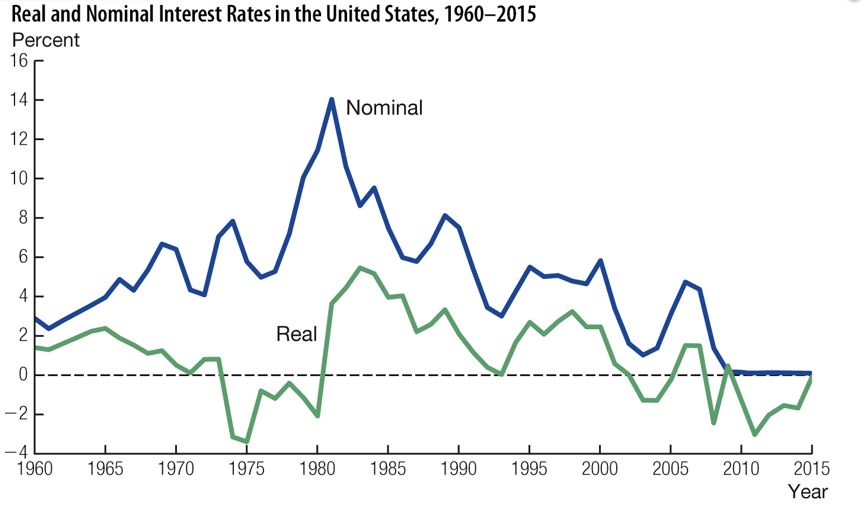
\includegraphics[scale=.5]{nominal_real_interest_rates}
\end{figure}
\end{frame}



\section{Short-Run Macroeconomics}


\begin{frame}
\frametitle{\: \: \: Short-Run Macroeconomics}
\toplinelarge
\begin{itemize}
\item The long-run model is a guide to how the economy behaves on average
\begin{itemize}
\vspace{.11in}
\item Determines potential output and long-run inflation
\end{itemize}
\vspace{.11in}
\item Potential output
\begin{itemize}
\vspace{.11in}
\item Amount of production if all inputs were utilized at their long-run sustainable levels
\end{itemize}
\vspace{.11in}
\item At any given time, the economy is unlikely to exactly equal the long-run average
\vspace{.11in}
\item The short-run model:
\begin{itemize}
\vspace{.11in}
\item Determines current output and current inflation
\end{itemize}
\end{itemize}
\end{frame}

\begin{frame}
\frametitle{\: \: \: Short-Run Macroeconomics}
\toplinelarge
\begin{itemize}
\item Actual output is equal to the long-run trend plus short-run fluctuations:
\begin{eqnarray*}
\underbrace{\text{actual output}}_{Y_t}=\underbrace{\text{long-run trend}}_{\overline{Y}_t}+\underbrace{\text{short-run fluctuations}}_{\text{function of  }\widetilde{Y}_t}
\end{eqnarray*}
\begin{itemize}
\vspace{.11in}
\item Long-run trend: potential ouptut
\vspace{.11in}
\item Short-run fluctuations: deviations from $\overline{Y_t}$
\end{itemize}
\end{itemize}
\end{frame}

\begin{frame}
\frametitle{\: \: \: Short-Run Macroeconomics}
\toplinelarge
\begin{itemize}
\item ``De-trended output'' or short-run output:
\begin{itemize}
\vspace{.11in}
\item The difference in actual and potential output, expressed as a percentage of potential output
\end{itemize}
\begin{eqnarray*}
\widetilde{Y}_t=\frac{Y_t-\overline{Y}_t}{\overline{Y}_t}
\end{eqnarray*}
\end{itemize}
\end{frame}



\begin{frame}
\frametitle{\: \: \: Short-Run Macroeconomics}
\toplinelarge
\begin{columns}
\begin{column}{0.5\linewidth}
\centering
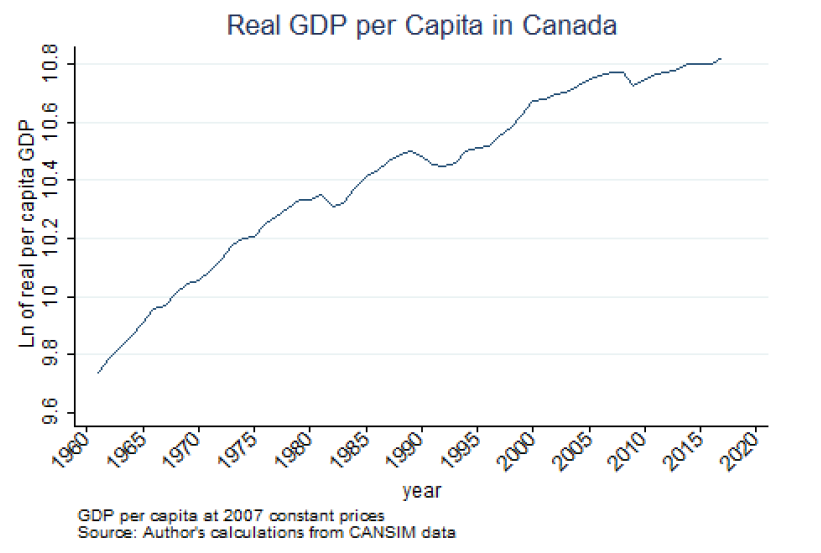
\includegraphics[scale=.25]{GDP_Canada}
\end{column}
\begin{column}{0.5\linewidth}
\centering
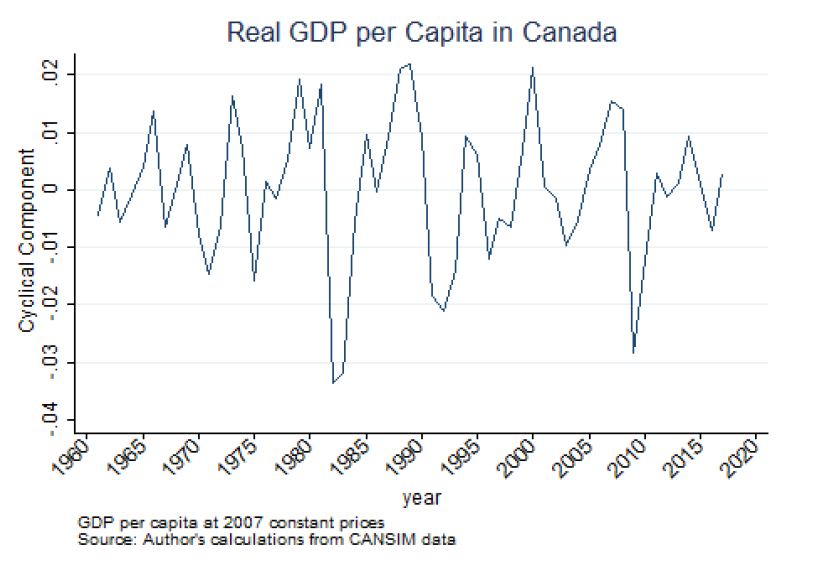
\includegraphics[scale=.25]{SR_GDP_Canada}
\end{column}
\end{columns}
\end{frame}

\begin{frame}
\frametitle{\: \: \: Economics Fluctuations and Unemployment}
\toplinexlarge
\begin{columns}
\begin{column}{0.5\linewidth}
\centering
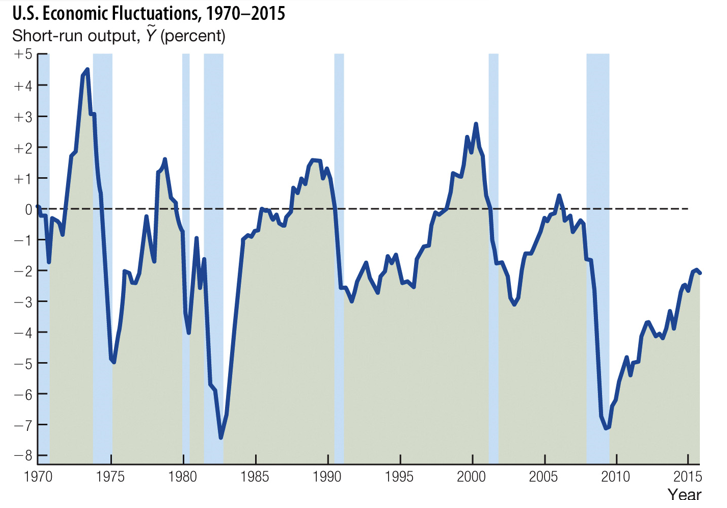
\includegraphics[scale=.3]{US_econ_fluctuations}
\end{column}
\begin{column}{0.5\linewidth}
\centering
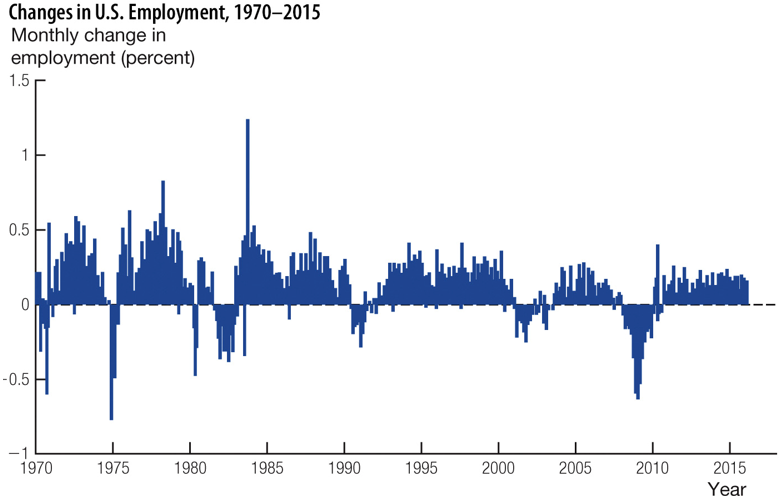
\includegraphics[scale=.3]{US_unemployment}
\end{column}
\end{columns}
\begin{itemize}
\item Recessions are very costly: 
\begin{itemize}
\vspace{.11in}
\item E.g. during a typical recessions GDP per households is around $\$12,000$ below potential output
\vspace{.11in}
\item Unemployment has long-run negative effects on the population.
\end{itemize}
\end{itemize}
\end{frame}




\begin{frame}
\frametitle{\: \: \: Inflation in the Short Run}
\toplinemedium
\begin{columns}
\begin{column}{0.6\linewidth}
\centering
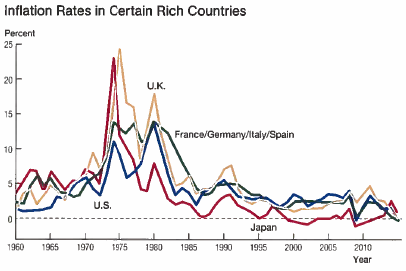
\includegraphics[scale=.8]{inflation}
\end{column}
\begin{column}{0.4\linewidth}
\begin{itemize}
\item Inflation increases during economic booms
\vspace{.11in}
\item Inflation decreases during recessions
\end{itemize}
\end{column}
\end{columns}
\end{frame}


\begin{frame}
\frametitle{\: \: \: Output-Inflation Trade-off}
\toplinelarge
\begin{itemize}
\item The Phillips Curve denotes the output-inflation trade-off:
\end{itemize}
\vspace{.13in}
\centering
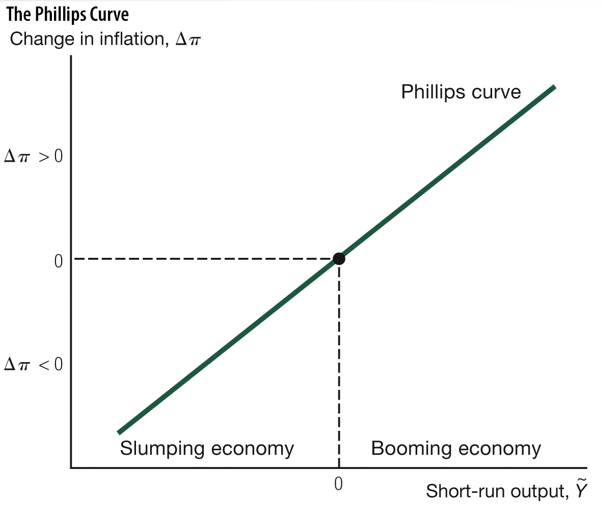
\includegraphics[scale=.5]{phillips_curve}
\end{frame}

\begin{frame}
\frametitle{\: \: \: Phillips Curve in the US}
\toplinelarge
\centering
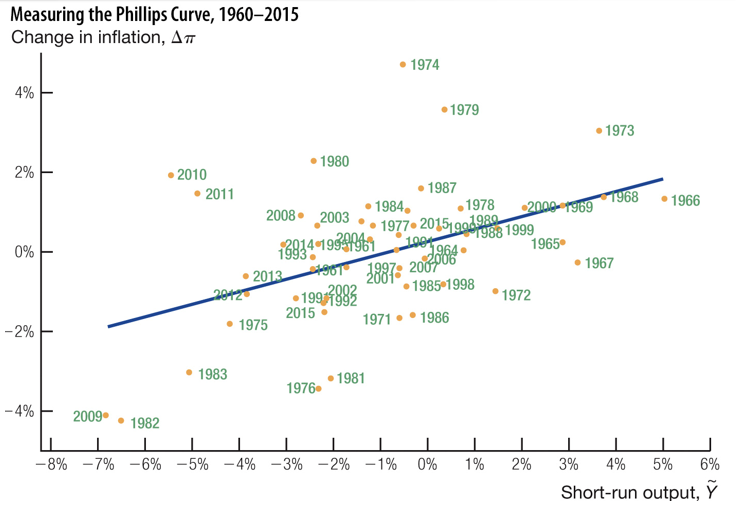
\includegraphics[scale=.5]{US_phillips}
\end{frame}


\begin{frame}
\frametitle{\: \: \: The Basis of the Short-Run Model}
\toplinelarge
\begin{itemize}
\item The economy is constantly being hit by shocks that cause fluctuations in economic activity
\begin{itemize}
\vspace{.11in}
\item Positive shocks increase economic activity beyond its natural rate, which results inflation.
\vspace{.11in}
\item Negative shocks decrease economic activity below its natural rate, which results in recessions.
\end{itemize}
\vspace{.11in}
\item Government through fiscal and monetary policy attempts to neutralize the effects of the shocks.
\vspace{.11in}
\item This creates a constant cycle of boom and bust.
\begin{itemize}
\vspace{.11in}
\item  The duration and severity depends on the shock and government's reaction to the shock.
\end{itemize} 
\end{itemize}
\end{frame}

\begin{frame}
\frametitle{\: \: \: Economic Activity and Unemployment}
\toplinelarge
\begin{itemize}
\item The Short-Run Model analyzes fluctuations in output and not in unemployment
\vspace{.11in}
\item There is a direct connection between unemployment and output, known as Okun's Law:
\begin{eqnarray*}
u-\overline{u}=-\frac{1}{2} \: \: \: \widetilde{Y}
\end{eqnarray*}
\begin{itemize}
\item $u$: current rate of unemployment 
\vspace{.11in}
\item $\overline{u}$: natural rate of unemployment
\vspace{.11in}
\item $\widetilde{Y}$: short-run output
\end{itemize}
\end{itemize}
\end{frame}

\begin{frame}
\frametitle{\: \: \: Okun's Law in the US}
\toplinemedium
\centering
\includegraphics[scale=.5]{okun_law}
\end{frame}

\begin{frame}
\frametitle{\: \: \: Preview of the Short-Run Model}
\toplinelarge
In the remainder of the semester:
\begin{enumerate}
\item We will carefully derive the IS-MP model and study the effects of shocks and government stabilization policy in this framework.
\vspace{.11in}
\item Afterward, we will study the connection between the IS-MP model and the Phillips curve.
\vspace{.11in}
\item Finally, we will put all the parts together and derive a model of the short-run economy, AS-AD, that simulates the periods of boom and bust that characterize modern economies.
\end{enumerate}
\end{frame}

\section{The Goods Market in the Short Run}

\begin{frame}
\frametitle{\: \: \: Introduction}
\toplinesmall
\begin{itemize}
\item Fluctuations in output around its potential level arise from aggregate demand variations.
\vspace{.11in}
\item In this lecture, I introduce a simple model of aggregate demand to study how output is determined:
\begin{itemize}
\vspace{.11in}
\item There are two key variables:
\begin{itemize}
\vspace{.11in}
\item Aggregate expenditure= $C+I+G+X-M$
\vspace{.11in}
\item Aggregate income= $Y$
\end{itemize}
\vspace{.11in}
\item In equilibrium, expenditure equals income:
\begin{eqnarray*}
Y=C+I+G+X-M
\end{eqnarray*}
\end{itemize}
\end{itemize}
\end{frame}

\begin{frame}
\frametitle{\: \: \: Components of aggregate expenditure}
\toplinexlarge
\begin{enumerate}
\item \textbf{Consumption:} Modelled as a function of income: 
\begin{eqnarray*}
\begin{array}{lll}
C=a_c+b_c \: \: Y &,& b_c<1 \text{  marginal propensity to consume}
\end{array}
\end{eqnarray*}
\vspace{.11in}
\item \textbf{Investment:} Modelled as a function of nominal interest rates:
\begin{eqnarray*}
\begin{array}{lll}
 I=a_i-b_i (R) &,& b_i<1
\end{array}
\end{eqnarray*}
\vspace{.11in}
\item \textbf{Government Expenditure:} Modelled as exogenous: $G=\overline{G}$
\vspace{.19in}
\item \textbf{Net Exports:} Modelled as exogenous: $NX=\overline{NX}=\overline{X}-\overline{M}$
\end{enumerate}
\end{frame}

\begin{frame}
\frametitle{\: \: \: Equilibrium in the Goods Market}
\toplinexlarge
\begin{itemize}
\item In equilibrium, Agg expenditure=Agg. output
\vspace{.16in}
\begin{eqnarray*}
\begin{array}{ll}
                   & Y=C+I+G+X-M \\ [3ex]
\Rightarrow & Y=a_c+b_c \: \: Y + a_i-b_i (R) + \overline{G}+\overline{X}-\overline{M} \\ [3ex]
\Rightarrow & Y=\underbrace{\left[\frac{1}{1-b_c}\right]}_{\text{multiplier}}* \left[a_c+ a_i-b_i (R) + \overline{G}+\overline{X}-\overline{M}\right] \\ [3ex]
\end{array}
\end{eqnarray*}
\end{itemize}
\end{frame}

\begin{frame}
\frametitle{\: \: \: The Keynesian Cross}
\toplinemedium
\begin{figure}
\centering
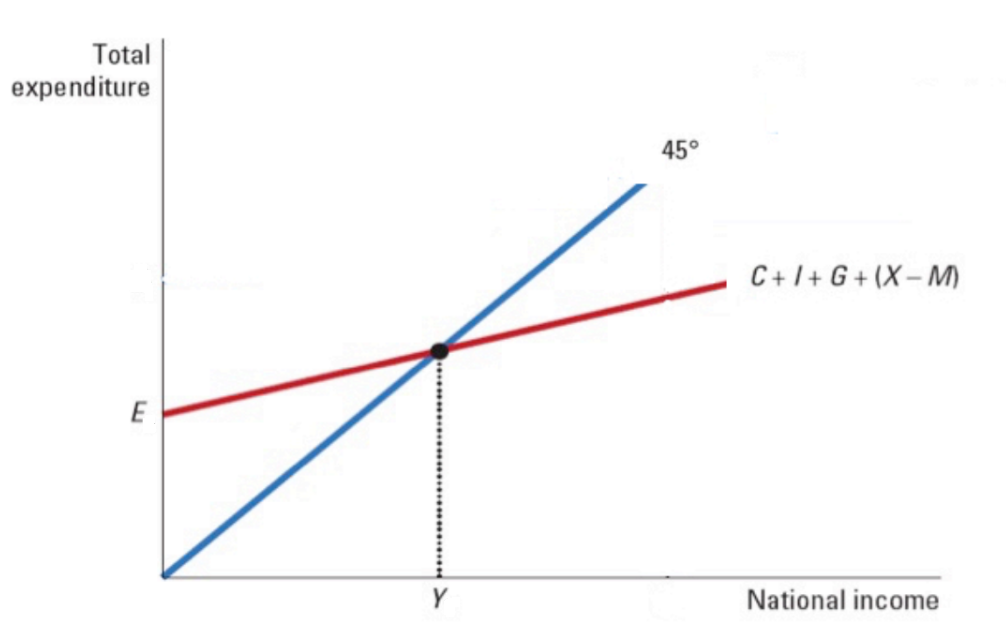
\includegraphics[scale=.5]{keynesian_cross}
\end{figure}
\end{frame}

\begin{frame}
\frametitle{\: \: \: Equilibrium in the Goods Market -- Revisited }
\toplinexlarge
\begin{columns}
\begin{column}{0.5\linewidth}
When $E>Y$, there is excess demand
\begin{itemize}
\item Firms increase production
\item Excess demand falls
\end{itemize}
\end{column}
\begin{column}{0.5\linewidth}
\begin{figure}
\centering
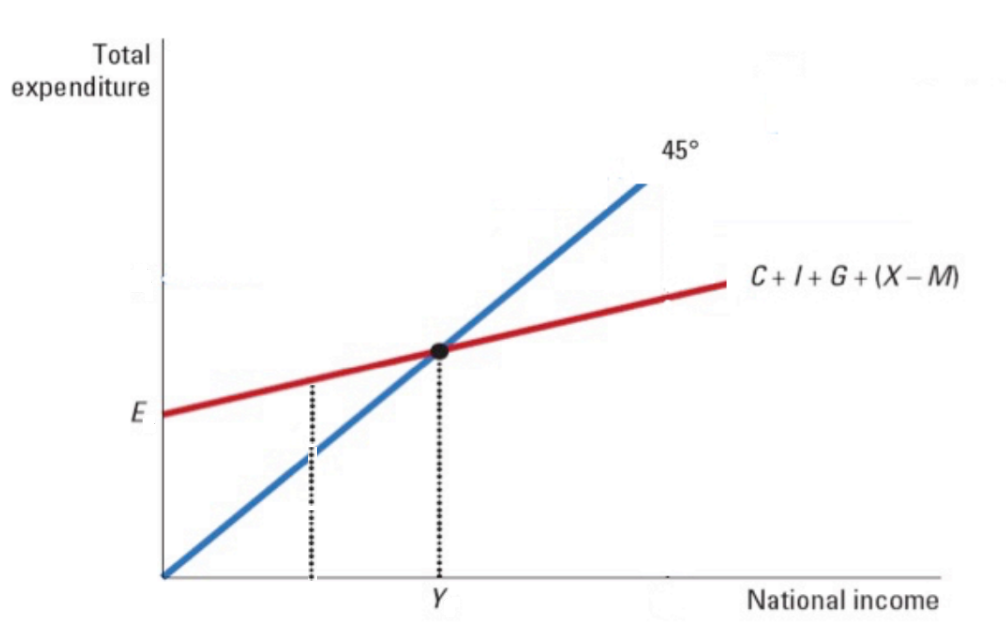
\includegraphics[scale=.23]{keynesian_cross_1}
\end{figure}
\end{column}
\end{columns}
\begin{columns}
\begin{column}{0.5\linewidth}
When $E<Y$, there is excess supply
\begin{itemize}
\item Firms decrease production
\item Excess supply falls
\end{itemize}
\end{column}
\begin{column}{0.5\linewidth}
\begin{figure}
\centering
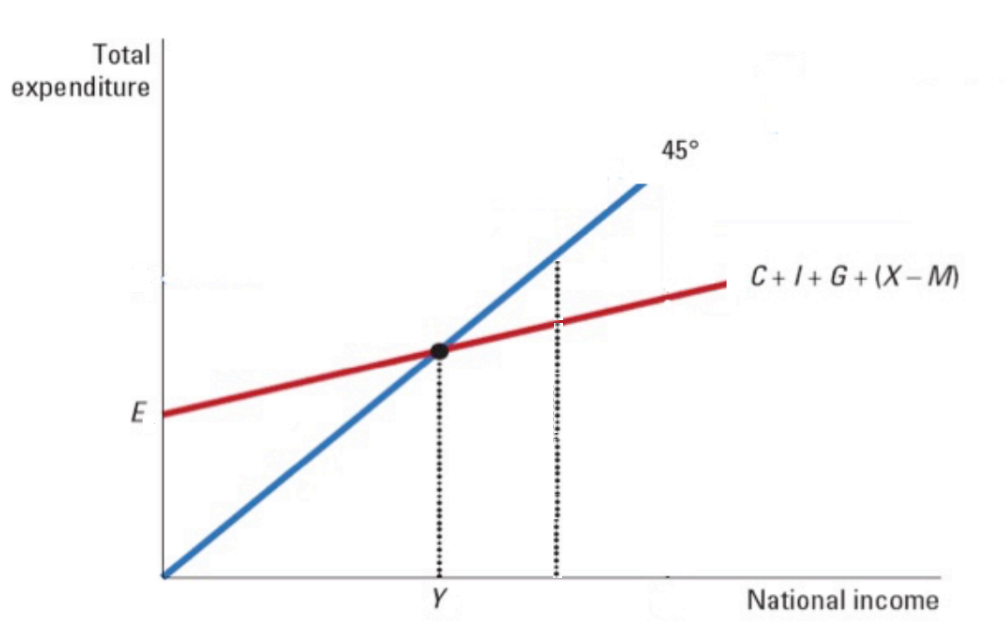
\includegraphics[scale=.23]{keynesian_cross_2}
\end{figure}
\end{column}
\end{columns}
\end{frame}


\begin{frame}
\frametitle{\: \: \: Changes in expenditure and the multiplier}
\toplinexlarge
\begin{figure}
\centering
\caption{Exogenous increase in $G$ from $\overline{G}$ to $\overline{G}'$}
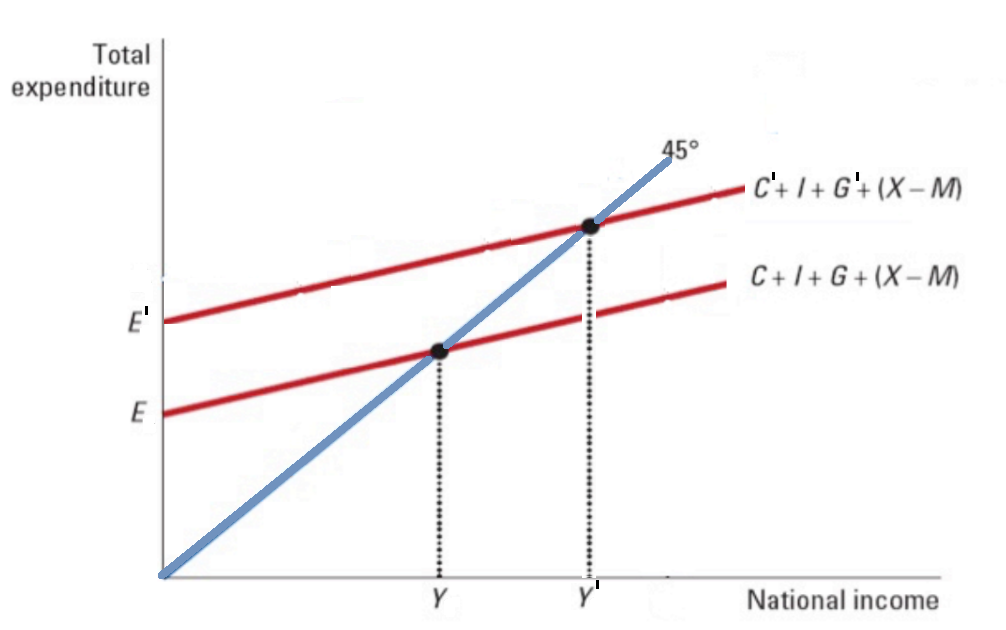
\includegraphics[scale=.45]{keynesian_cross_change_1}
\end{figure}
\end{frame}

\begin{frame}
\frametitle{\: \: \: Changes in expenditure and the multiplier}
\toplinexlarge
\begin{figure}
\centering
\caption{Exogenous increase in $G$ from $\overline{G}$ to $\overline{G}'$}
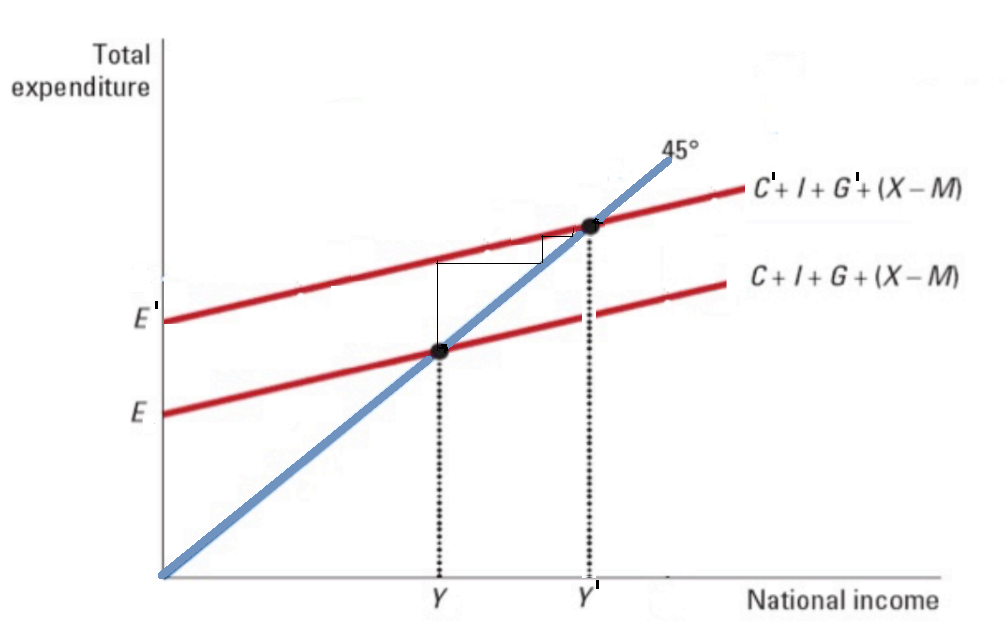
\includegraphics[scale=.45]{keynesian_cross_change_2}
\end{figure}
\end{frame}

\begin{frame}
\frametitle{\: \: \: Deriving the IS-curve}
\toplinemedium
\begin{figure}
\centering
\caption{IS curve: $Y=\left[\frac{1}{1-b_c}\right]* \left[a_c+ a_i-b_i (R) + \overline{G}+\overline{X}-\overline{M}\right]$}
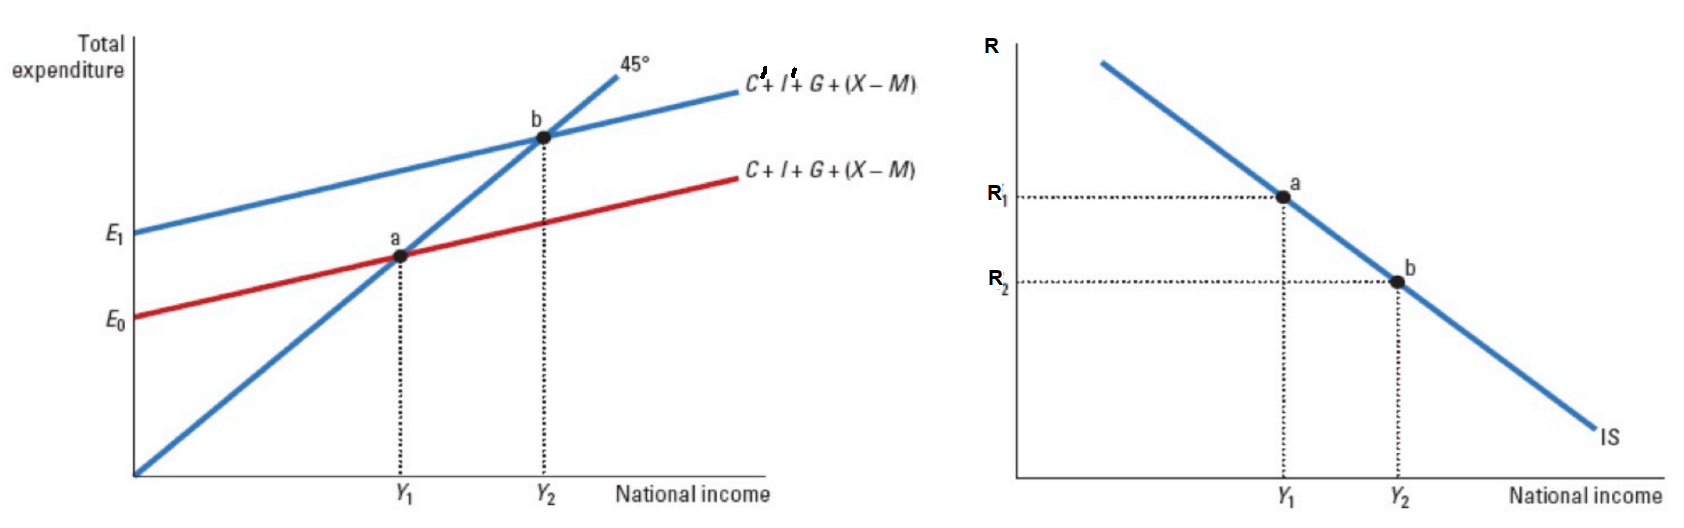
\includegraphics[scale=.25]{deriving_IS_curve}
\end{figure}
\end{frame}

\begin{frame}
\frametitle{\: \: \: Parametric Shifts in the IS-curve}
\toplinelarge
\begin{figure}
\centering
\caption{IS curve: $Y=\left[\frac{1}{1-b_c}\right]* \left[a_c+ a_i-b_i (R) + \overline{G}+\overline{X}-\overline{M}\right]$}
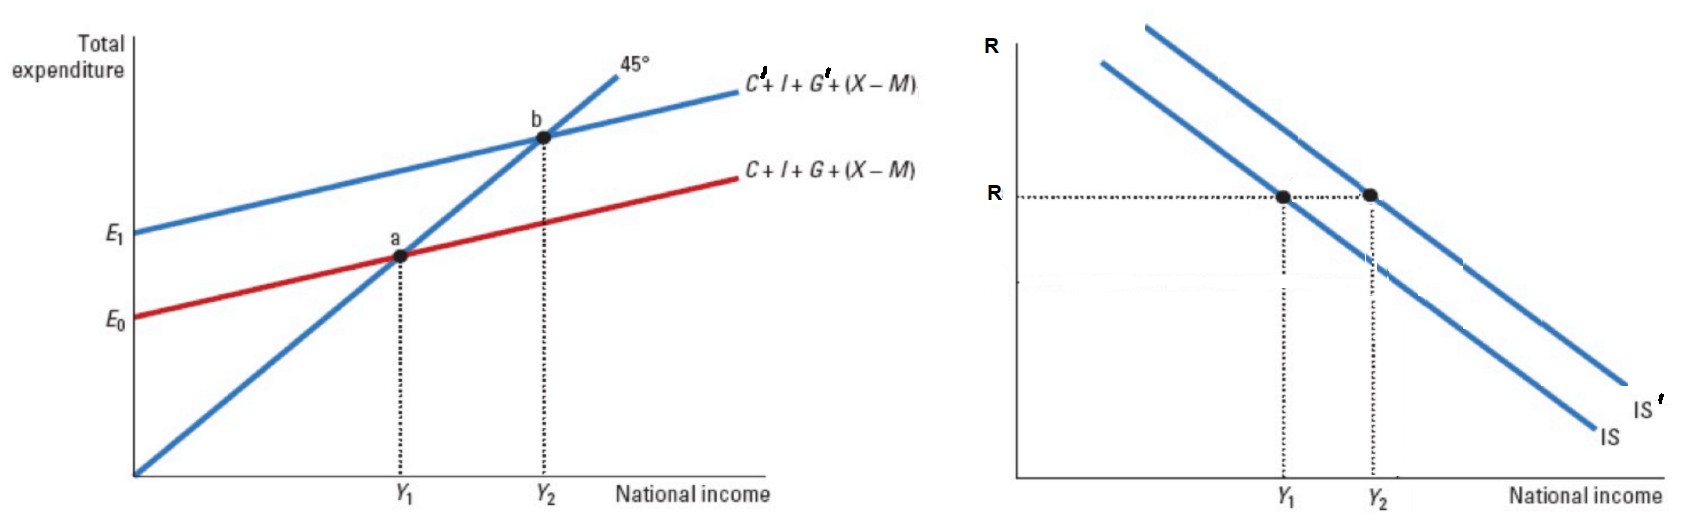
\includegraphics[scale=.25]{parametric_IS_curve}
\end{figure}
\end{frame}


\begin{frame}
\frametitle{\: \: \: Change of scale}\label{scale}
\toplinemedium
\begin{itemize}
\item We are interested in $\widetilde{Y}_t=\frac{Y_t-\overline{Y}}{\overline{Y}}$, so we are going to rewrite the equilibrium as follows:
\begin{eqnarray*} 
\widetilde{Y}_t=\left[\frac{1}{1-b_c}\right]* \left[\overline{a}-\overline{b}_i (R_t-\overline{r}) \right]-1
\end{eqnarray*}
\begin{itemize}
\item $\overline{a}=\frac{a_c}{\overline{Y}}+\frac{a_i}{\overline{Y}}-\frac{b_i}{\overline{Y}}\overline{r}+\frac{\overline{G}}{\overline{Y}}+\frac{\overline{X}}{\overline{Y}}-\frac{\overline{M}}{\overline{Y}}$
\vspace{.16in}
\item $\overline{b}_i=\frac{b_i}{\overline{Y}}$
\end{itemize}
\vspace{.16in}
\item If all exogenous variables are at their long-run equilibrium: 
\begin{eqnarray*}
\begin{array}{lll}
\left[\frac{1}{1-b_c}\right]*\overline{a}=1 &\Rightarrow &\widetilde{Y}_t=\left[\frac{1}{1-b_c}\right][-\overline{b}_i*(R_t-\overline{r})]
\end{array}
\end{eqnarray*}
\end{itemize}
\hyperlink{algebra}{\beamerbutton{Algebra}}
\end{frame}

\begin{frame}
\frametitle{\: \: \: IS-curve with new scale}
\toplinelarge
\begin{figure}
\centering
\caption{IS-curve:$\widetilde{Y}_t=\left[\frac{1}{1-b_c}\right]* \left[\overline{a}-\overline{b}_i (R_t-\overline{r}) \right]-1$, $\overline{a}\left[\frac{1}{1-b_c}\right]=1$}
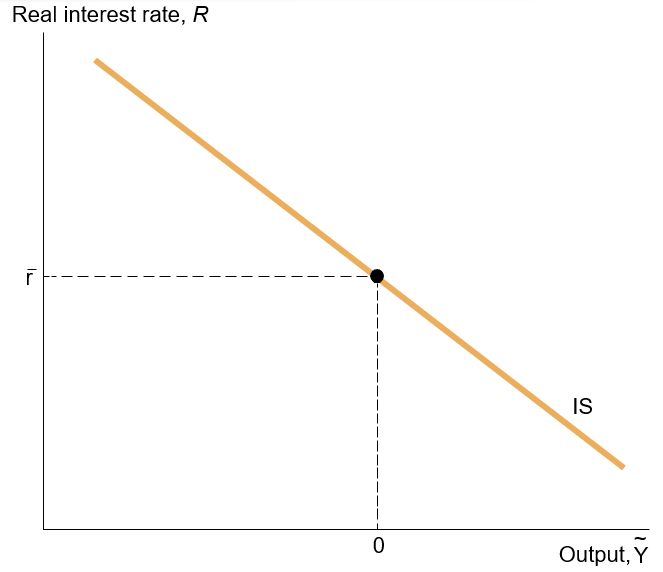
\includegraphics[scale=.5]{IS_curve}
\end{figure}
\end{frame}


\begin{frame}
\frametitle{\: \: \: Changes in the real interest rate}
\toplinelarge
\begin{figure}
\centering
\caption{IS-curve:$\widetilde{Y}_t=\left[\frac{1}{1-b_c}\right]* \left[\overline{a}-\overline{b}_i (R_t-\overline{r}) \right]-1$, $\overline{a}\left[\frac{1}{1-b_c}\right]=1$}
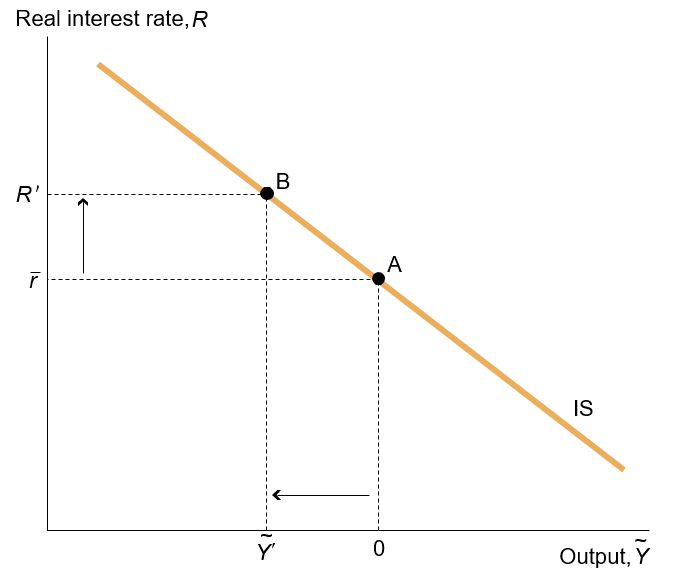
\includegraphics[scale=.5]{IS_curve_interest_rate}
\end{figure}
\end{frame}

\begin{frame}
\frametitle{\: \: \: Temporary Aggregate Demand Shock}
\toplinelarge
\begin{figure}
\centering
\caption{IS-curve:$\widetilde{Y}_t=\left[\frac{1}{1-b_c}\right]* \left[\overline{a}-\overline{b}_i (R_t-\overline{r}) \right]-1$, $\overline{a}\left[\frac{1}{1-b_c}\right]=1$, $\overline{a}'>(1-b_c)$}
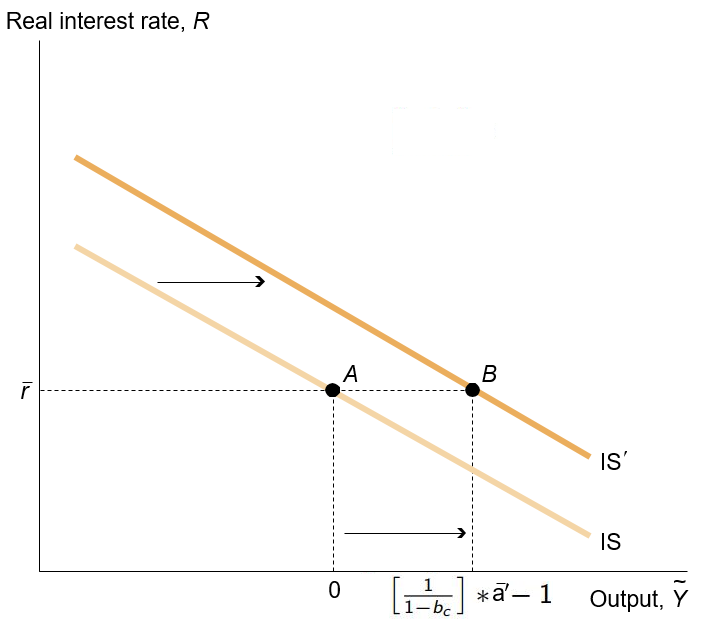
\includegraphics[scale=.39]{aggregate_demand_shock}
\end{figure}
\end{frame}

\begin{frame}
\frametitle{\: \: \: Permanent Aggregate Shock}
\toplinelarge
\begin{itemize}
\item Permanent shocks impact potential output and originate from the production side of the economy, which have two effects:
\begin{enumerate}
\vspace{.11in}
\item Permanent shocks affect demand parameters, which affect both long- and short-run output levels equally.
\vspace{.11in}
\item Permanent production shocks affect the $MPK$
\begin{itemize}
\vspace{.11in}
\item This has no effect in the long-run because $\overline{r}=MPK$
\vspace{.16in}
\item This results in output overshooting in the SR as the economy adjusts to its new potential output.
\end{itemize}
\end{enumerate}
\end{itemize}
\end{frame}

\begin{frame}
\frametitle{\: \: \: E.g. Permanent TFP shock}
\toplinelarge
\begin{figure}
\centering
\caption{IS-curve:$\widetilde{Y}_t=\left[\frac{1}{1-b_c}\right]* \left[\overline{a}-\overline{b}_i (R_t-\overline{r}) \right]-1$, $\overline{a}\left[\frac{1}{1-b_c}\right]=1$, $\overline{r}'>\overline{r}$}
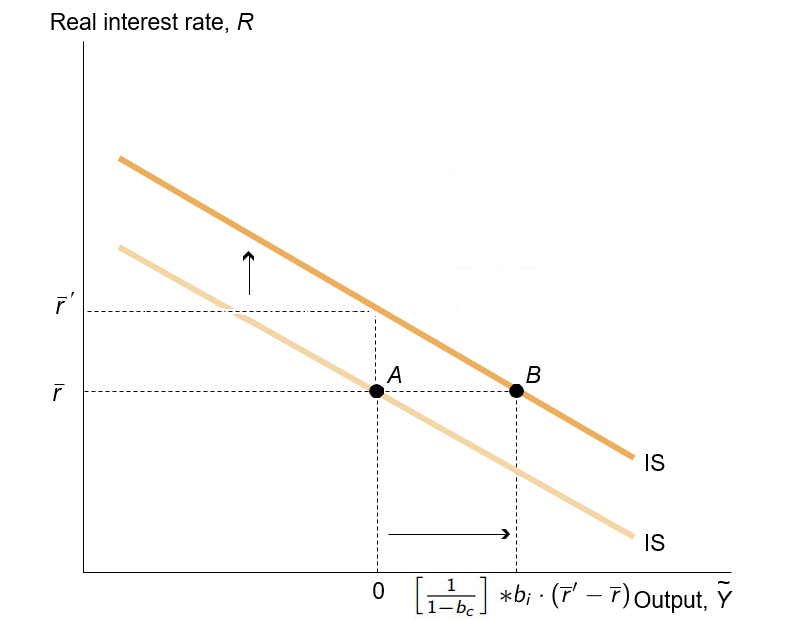
\includegraphics[scale=.39]{permanent_shock}
\end{figure}
\end{frame}





\section{Appendix}

\begin{frame}
\frametitle{\: \: \: Change of Scale: Derivation (part 1)}\label{algebra}
\toplinelarge
\begin{itemize}
\item We begin with the solution to $Y_t$ in the SR equilibrium:
\begin{eqnarray*}
Y_t=\frac{1}{1-b_c} \left(a_c+a_i-b_i \: R_t +\overline{G}+\overline{X}-\overline{M}\right)
\end{eqnarray*}
\item We first divide both sides by the long-run output level $\overline{Y}$ and then subtract one from both sides:
\begin{eqnarray*}
\frac{Y_t}{\overline{Y}}-1=\underbrace{\frac{Y_t-\overline{Y}}{\overline{Y}}}_{\widetilde{Y}_t}=\frac{1}{1-b_c} \left(\frac{a_c}{\overline{Y}}+\frac{a_i}{\overline{Y}}-\frac{b_i}{\overline{Y}} \: R_t +\frac{\overline{G}}{\overline{Y}}+\frac{\overline{X}}{\overline{Y}}-\frac{\overline{M}}{\overline{Y}}\right)-1
\end{eqnarray*}
\item We add and subtract $\frac{b_i}{\overline{Y}} \: \overline{r}$:
\begin{eqnarray*}
\widetilde{Y}_t=\frac{1}{1-b_c} \left(\frac{a_c}{\overline{Y}}+\frac{a_i}{\overline{Y}}-\frac{b_i}{\overline{Y}} \: R_t +\frac{b_i}{\overline{Y}} \: \overline{r}-\frac{b_i}{\overline{Y}} \: \overline{r}+ \frac{\overline{G}}{\overline{Y}}+\frac{\overline{X}}{\overline{Y}}-\frac{\overline{M}}{\overline{Y}}\right)-1
\end{eqnarray*}
\end{itemize}
\end{frame}

\begin{frame}
\frametitle{\: \: \: Change of Scale: Derivation (part 2)}
\toplinelarge
\begin{itemize}
\item We rearrange terms to obtain:
\begin{eqnarray*}
\begin{array}{l}
\widetilde{Y}_t=\frac{1}{1-b_c}\left[\overline{a}-\overline{b}_i \left(R_t-\overline{r}\right)\right]-1  \\
\text{where,}\\
\overline{a}=\frac{a_c}{\overline{Y}}+\frac{a_i}{\overline{Y}}-\frac{b_i}{\overline{Y}} \: \overline{r} + \frac{\overline{G}}{\overline{Y}}+\frac{\overline{X}}{\overline{Y}}-\frac{\overline{M}}{\overline{Y}}\\
\text{and,}\\
\overline{b_i}=\frac{b_i}{\overline{Y}} \\
\text{and,}
\overline{Y}=\frac{1}{1-b_c} \left(a^{LR}_c+a^{LR}_i-b^{LR}_i \: \overline{r} +\overline{G}^{LR}+\overline{X}^{LR}-\overline{M}^{LR}\right)
\end{array}
\end{eqnarray*}
\item From the previous equation, we can see that if all parameters in the SR are equal their long-run levels:
\begin{eqnarray*}
\overline{a}=\frac{a^{LR}_c+a^{LR}_i-b^{LR}_i \: \overline{r}+\overline{G}^{LR}+\overline{X}^{LR}-\overline{M}^{LR}}{\frac{1}{1-b_c} \left(a^{LR}_c+a^{LR}_i-b^{LR}_i \: \overline{r} +\overline{G}^{LR}+\overline{X}^{LR}-\overline{M}^{LR}\right)}
\end{eqnarray*}
\item Solving for this results in: $\overline{a}=1-b_c$
\end{itemize}
\hyperlink{scale}{\beamerbutton{Back}}
\end{frame}


\end{document}

